\renewcommand{\newCommandChapterTitle}{Clasificación con One-Class SVM}
\chapter{\newCommandChapterTitle}
\markright{\hfill \thechapter. \newCommandChapterTitle}
\label{chap:p3_concepts_ocsvm}


La detección de anomalías en peticiones \gls{acr3:http} puede ser encarada
como un problema de clasificación. Nosotros empleamos la estrategia
\gls{acr3:occ} \citep{khan2009survey} % from section 1 - introduction
para la detección de anomalías en nuestro detector \gls{acr3:name}.
Para este fin utilizamos el clasificador \gls{acr3:ocsvm}, que es una
herramienta del área de \gls{acr3:ml}.

Iniciaremos este capítulo explicando algunos conceptos sobre problemas
de clasificación y las herramientas utilizadas para resolverlos, luego
describimos el funcionamiento del \gls{acr3:ocsvm} y mostramos cómo este
clasificador es utilizado para la detección de peticiones anómalas
dentro de nuestro \gls{acr3:waf}.


\section{Conceptos sobre problemas de clasificación}

La detección de anomalías puede ser encarada como un problema de
clasificación. En este tipo de problemas se busca clasificar las muestras
en varios grupos o clases. Acá se observan dos fases, una de entrenamiento
y otra de detección o clasificación.
En este contexto se habla de aprendizaje supervisado si se especifican
todas las clases posibles de antemano, usando solamente muestras para el
entrenamiento de las que se conocen sus clases; muestras nuevas serán
asignadas a la clase a la que más se parezcan en la fase de detección.
En cambio, se habla de aprendizaje no supervisado cuando no se provee
muestras con clases conocidas de antemano y la herramienta utilizada
debe tratar de encontrar las clases presentes en las muestras
\citep{torranoGimenez2015study}. % from section 2.4.2 - ML
También se puede dar el caso de que se conozca las clases de solamente
algunas de las muestras, o que se tenga únicamente muestras de una clase
conocida pero no se tenga muestras de las demás clases; en estos casos
se puede hablar de aprendizaje semi-supervisado
\citep{aggarwal2013outlier}. % from section 7.4 - Semi-Supervision

Aplicado a un \gls{acr3:waf}, se puede usar clasificación supervisada,
definiendo una clase para los mensajes normales y otra clase (o también
varias otras clases) para los mensajes anómalos.
Un primer desafío con este abordaje es que se necesita volver a entrenar
el clasificador cuando aparece un nuevo tipo de anomalía. Si no se vuelve
a entrenarlo con muestras que contengan los nuevos tipos de anomalías, es
posible que una anomalía sea clasificada equivocadamente como un mensaje
normal en el caso de una anomalía nueva que no se ajusta suficientemente
a las clases de anomalías con las cuales el clasificador fue entrenado
anteriormente.
Un segundo desafío con este abordaje es la necesidad de obtener muestras
de todos los tipos de anomalías conocidas para poder realizar un
entrenamiento completo.

Una de las estrategias utilizadas para abordar estos dos desafíos es
la clasificación de una sola clase (\gls{acr3:occ} - \textit{One-Class Classification}),
que corresponde al tipo semi-supervisado
\citep{khan2009survey}. % from section 1 - introduction
Se busca definir una sola clase, la clase conocida, y clasificar las
muestras de acuerdo a si pertenecen o no a dicha clase. La fase de
entrenamiento utiliza solamente muestras de la clase conocida, con la
finalidad de que en la fase de detección las muestras que no se ajusten
a la clase conocida sean clasificadas como no perteneciente a la misma.
Esta característica permite que el clasificador no necesite ser entrenado
de vuelta con la aparición de novedosas muestras que no pertenecen a la
clase conocida.
Esta estrategia ha sido utilizada con éxito en varias áreas, como por
ejemplo en la detección de spam, reconocimiento de rostros, detección
de fallas en maquinarias, entre otros
\citep{khan2014one}. % from section 4.3.2 - application domains

Aplicado a un \gls{acr3:waf}, la clase conocida esta conformada solamente
por los mensajes normales y todos los tipos de anomalías que representan
los distintos tipos de ataques no pertenecerán a dicha clase. Para ser
consistentes con la terminología del área de seguridad, las anomalías o
ataques son las muestras positivas, que no pertenecerán a la clase conocida
de los mensajes normales (que son las muestras negativas).


\section{Herramientas del área de \textit{Machine Learning}}

Para realizar la detección de anomalías en el contexto de problemas de
clasificación se puede utilizar varias estrategias y herramientas.
Una opción es emplear herramientas estadísticas, como podemos ver en
los trabajos \citep{kruegel2003anomaly}, \citep{gimenez2015tfg} y
\citep{torranoGimenez2015study}.
Otra opción son herramientas del área de aprendizaje de máquinas
(\gls{acr3:ml} - \textit{Machine Learning}) para tratar de detectar
las anomalías; podemos ver esto en los trabajos \citep{sommer2010outside},
\citep{buczak2016survey}, \citep{parhizkar2015oc}
y \citep{torranoGimenez2015study}.

En este trabajo nosotros elegimos la opción de utilizar herramientas
del área de \gls{acr3:ml} para tratar de detectar las anomalías. Este
tipo de herramientas han sido empleadas con mucho éxito en varias áreas
de la computación, como por ejemplo en sistemas de recomendación de
productos, clasificación de imágenes, detección de rostros, reconocimiento
óptico de caracteres, detección de anomalías, entre otros
\citep{torranoGimenez2015study}. % from section 2.4.2 - ML
Podemos ver ejemplos de estos en los trabajos \citep{sommer2010outside},
\citep{buczak2016survey}, \citep{parhizkar2015oc} y
\citep{torranoGimenez2015study}.

Los algoritmos o herramientas utilizados en \gls{acr3:ml} son muy diversos,
como por ejemplo
árboles de decisiones \citep{torranoGimenez2015study}, % from section 2.4.2 - ML
redes neuronales \citep{corchado2011neural},
algoritmos genéticos \citep{abadeh2011design},
entre otros \citep{torranoGimenez2015study}. % from section 2.4.2 - ML
Una de estas herramientas, que ha sido utilizada con mucho éxito en las
tareas de clasificación, es la máquina de vectores de soporte
(\gls{acr3:svm} - \textit{Support Vector Machine}). Una versión modificada
del \gls{acr3:svm} ha sido propuesta como una de varias alternativas
para afrontar tareas de \gls{acr3:occ} \citep{scholkopf2001estimating}.
Varios investigadores ya han empleado exitosamente este clasificador
\gls{acr3:ocsvm} en problemas de distintas áreas, como por ejemplo en
clasificación de textos, clasificación de rostros en imágenes, detección
de spam, detección de fallas en máquinas, detección de anomalías, entre
otros \citep{khan2014one}. % from section 4.3.2 - application domains


\section{Funcionamiento del One-Class SVM}

Los \gls{acr3:svm}s son clasificadores binarios de aprendizaje supervisado.
Estos clasificadores tratan de separar de forma óptima las dos clases
utilizando un hiperplano, buscando minimizar la penalización incurrida
por la clasificación incorrecta de alguna de las muestras de entrenamiento.
El nombre se debe a que habrá un subconjunto de muestras que determinarán
la posición del hiperplano separador; estas muestras son los vectores de
soporte que determinan la separación de las clases
\citep{aggarwal2013outlier}. % from section 7.2.1.2 - weighting methods - SVMs

Una versión modificada del \gls{acr3:svm} ha sido propuesta como una de
varias alternativas para afrontar tareas de \gls{acr3:occ}
\citep{scholkopf2001estimating}.
Este clasificador \gls{acr3:ocsvm} solamente recibe muestras de la clase
conocida en la fase de entrenamiento y trata de trazar un hiperplano que
separe las muestras del origen de coordenadas. Se busca maximizar la
distancia del hiperplano al origen, tratando de minimizar al mismo tiempo
la cantidad de muestras situadas en el mismo lado del hiperplano que el
origen. Las muestras del lado opuesto al origen serán consideradas
pertenecientes a la clase conocida, las demás no pertenecerán a dicha
clase \citep{khan2009survey}. % from section 3.2 - algorithm used - OCSVM

A continuación presentamos las ecuaciones que definen el comportamiento
del clasificador \gls{acr3:ocsvm}. Para eso, vamos a utilizar la notación
de detección de anomalías con peticiones \gls{acr3:http} que presentamos
en el capítulo anterior, a modo de que las ecuaciones se ajusten a la
nomenclatura empleada en este trabajo.


\subsection{Fase de entrenamiento}

En esta fase, el clasificador \gls{acr3:ocsvm} traza un hiperplano que
separa las muestras de entrenamiento del origen.
En nuestro contexto de detección de anomalías, nuestro \gls{acr3:waf}
realiza un preprocesamiento de datos en el cual las peticiones \gls{acr3:http}
son representadas por medio de vectores numéricos de \textit{features}
\gls{sim3:fij}. Como explicamos en el capítulo anterior, las peticiones
disponibles para el entrenamiento son agrupadas por método y \gls{acr3:url},
y de cada uno de esos grupos \gls{sim3:gi} se construye una matriz
\gls{sim3:mi}. Esa matriz tendrá una cantidad de filas igual a la cantidad
de peticiones en \gls{sim3:gi} y una cantidad de columnas igual a la
dimensión de los vectores \gls{sim3:fij} del grupo. Después se entrena
un clasificador por grupo, usando la matriz \gls{sim3:mi} para
dicho entrenamiento.


\subsubsection{Formulación del problema de optimización}

El \gls{acr3:ocsvm} busca un hiperplano que separa las muestras (en
nuestro caso, los vectores de \textit{features} \gls{sim3:fij}) del origen.
Este hiperplano puede ser expresado como lo muestra la
\autoref{eq:ocsvm:hyperplane1}
\citep{parhizkar2015oc}. % from section II.A - one class SVM

\begin{equation}
    \label{eq:ocsvm:hyperplane1}
    \vec{w_{i}} \cdot \vec{x}
    \ - \
    \rho_{i}
    \ = \
    0
\end{equation}

En esta ecuación, \gls{sim3:wi} es el vector perpendicular al hiperplano,
$\vec{x}$ es un vector variable y \gls{sim3:rhoi} indica la distancia
del hiperplano al origen para el clasificador del grupo \gls{sim3:gi}.

Para obtener el hiperplano óptimo, se busca resolver el problema de
optimización de la \autoref{eq:ocsvm:min_problem_goal1}, sujeto a las
restricciones de la \autoref{eq:ocsvm:min_problem_restr1}
\citep{parhizkar2015oc}. % from section II.A - one class SVM

\begin{equation}
    \label{eq:ocsvm:min_problem_goal1}
    \min_{
        \vec{w_{i}}
        \ , \
        \rho_{i}
        \ , \
        \xi_{i}
    }
    \
    \frac{1}{2} \lVert {\vec{w_{i}}} \rVert^2
    \ - \
    \rho_{i}
    \ + \
    \frac{1}{\nu_{i} \lvert G_{i} \rvert} \sum_{j=1}^{\lvert G_{i} \rvert} \xi_{ij}
\end{equation}

\begin{equation}
    \label{eq:ocsvm:min_problem_restr1}
    \vec{w_{i}} \cdot \vec{f_{ij}} \geqslant \rho_{i} - \xi_{ij}
    \ , \quad
    \xi_{ij} \geqslant 0
    \ , \quad
    \forall j = 1,2, \dots, \lvert G_{i} \rvert
\end{equation}

Podemos notar dos parámetros fijos en la tarea de minimización de la
\autoref{eq:ocsvm:min_problem_goal1}; $\lvert G_{i} \rvert$ indica la
cantidad de muestras utilizadas para el entrenamiento del clasificador
y \gls{sim3:nui} es un parámetro que regula la fracción de muestras
situadas al mismo lado del hiperplano que el origen para el grupo
\gls{sim3:gi}. Esas muestras serán clasificadas como no pertenecientes
a la clase conocida y así, en el contexto de nuestro \gls{acr3:waf},
este parámetro puede ser considerado como la fracción aceptable de
falsos positivos para el entrenamiento (peticiones \gls{acr3:http}
normales detectadas equivocadamente como anomalías).
Por otro lado, el parámetro \gls{sim3:nui} puede ser de utilidad en caso
de que haya algunas muestras no pertenecientes a la clase conocida en
los datos de entrenamiento. Para esos casos, el clasificador puede dejar
ciertas muestras al mismo lado del hiperplano que el origen, obteniendo
de esta forma cierta robustez frente a la presencia de ruido en los
datos de entrenamiento
\citep{parhizkar2015oc}. % from section II.A - one class SVM

La tarea de minimización tiene tres variables para las cuales el clasificador
busca la combinación óptima; el vector \gls{sim3:wi} que define el hiperplano
del grupo, la distancia \gls{sim3:rhoi} del hiperplano al origen y en tercer
lugar la lista de valores de holgura \gls{sim3:slacki}, que indica las
penalizaciones incurridas por muestras situadas al mismo lado del hiperplano
que el origen (estas muestras serán falsos positivos)
\citep{parhizkar2015oc}. % from section II.A - one class SVM

Cada una de estas variables domina uno de los tres términos del problema
de minimización. El primer término esta gobernado por la norma $l_{2}$
del vector \gls{sim3:wi}, causando que el clasificador busque el menor
valor posible para dicha norma.
El segundo término consta de la distancia del hiperplano al origen pero
tomado con signo negativo, lo que provoca que el clasificador busque
maximizar dicha distancia. El último término indica la penalización total
incurrida por las muestras de entrenamiento situadas al mismo lado del
hiperplano que el origen (estas muestras serán falsos positivos), causando
que el clasificador trate de minimizar dichos casos
\citep{parhizkar2015oc}. % from section II.A - one class SVM

En las restricciones presentadas en la \autoref{eq:ocsvm:min_problem_restr1}
podemos observar que cada una de las muestras (en nuestro caso, los
vectores \gls{sim3:fij}) debe estar ubicada a una distancia mayor o igual
a $\rho_{i} - \xi_{ij}$ del origen. En el caso ideal, los valores de
holgura $\xi_{ij}$ para todas las muestras son 0, lo que significa que
ninguna de las muestras se encuentra del mismo lado del hiperplano que el
origen. En cambio, si alguna muestra de entrenamiento se encuentra en el
mismo lado que el origen (será un falso positivo), la holgura correspondiente
a esa muestra deberá tener un valor mayor a 0 para satisfacer las
restricciones, provocando que el problema de minimización tendrá una
penalización que debe considerar.
Esto otorga cierta flexibilidad al clasificador para balancear entre el
aumento de la distancia \gls{sim3:rhoi} (alejando el hiperplano del
origen) o la reducción de la cantidad de elementos en \gls{sim3:slacki}
con valores mayores a 0 (reduciendo la cantidad de falsos positivos)
\citep{parhizkar2015oc}. % from section II.A - one class SVM


\subsubsection{Transformación a espacios de dimensiones mayores}

Dependiendo del conjunto de muestras utilizadas para el entrenamiento,
el clasificador \gls{acr3:ocsvm} no siempre podrá encontrar un hiperplano
adecuado para separar las muestras del origen. Una solución a esta
situación es mapear las muestras a un espacio vectorial de dimensiones
mayores para encontrar un hiperplano separador en ese nuevo espacio
\citep{parhizkar2015oc}. % from section II.A - one class SVM
Esta transformación puede ser expresada como funciones
$\phi: \mathbb{R}^{n} \rightarrow \mathbb{R}^{m}$, que llevan las muestras
del espacio original $\mathbb{R}^{n}$ a otro espacio $\mathbb{R}^{m}$,
con $n \leq m$. El hiperplano trazado por el clasificador en el espacio
$\mathbb{R}^{m}$ puede quedar representado por una superficie no lineal
en el espacio original $\mathbb{R}^{n}$.

Para obtener esta transformación, se utiliza funciones $\phi$ para modificar
los vectores de muestras en las ecuaciones \ref{eq:ocsvm:hyperplane1} y
\ref{eq:ocsvm:min_problem_restr1}, obteniendo de esta forma las nuevas
ecuaciones \ref{eq:ocsvm:hyperplane2} y \ref{eq:ocsvm:min_problem_restr2}
\citep{parhizkar2015oc} % from section II.A - one class SVM
\citep{amer2013paper}. % from section 3.1 - Motivation of OneClassSVM
En estas ecuaciones, el vector \gls{sim3:wi} del hiperplano se encuentra
también en el nuevo espacio $\mathbb{R}^{m}$.
Cabe aclarar que la formulación del problema de minimización que presentamos
en la \autoref{eq:ocsvm:min_problem_goal1} no sufre modificaciones por la
introducción de esta transformación.

\begin{equation}
    \label{eq:ocsvm:hyperplane2}
    \vec{w_{i}} \cdot \phi(\vec{x})
    \ - \
    \rho_{i}
    \ = \
    0
\end{equation}

\begin{equation}
    \label{eq:ocsvm:min_problem_restr2}
    \vec{w_{i}} \cdot \phi(\vec{f_{ij}}) \geqslant \rho_{i} - \xi_{ij}
    \ , \quad
    \xi_{ij} \geqslant 0
    \ , \quad
    \forall j = 1,2, \dots, \lvert G_{i} \rvert
\end{equation}

En la \autoref{fig:ocsvm:svm_transformed_space} se puede observar un
ejemplo sencillo que ilustra como la transformación de las muestras a
otro espacio vectorial puede ayudar a trazar el hiperplano. Los círculos
rojos indican muestras de la clase conocida utilizadas en entrenamiento,
mientras que los cuadrados azules representan las muestras analizadas
durante la fase de detección que no pertenecen a la clase conocida.
Cabe aclarar que durante la fase de entrenamiento el clasificador no tiene
disponible los cuadrados azules para buscar el hiperplano óptimo.
Se puede notar que el clasificador logra trazar un hiperplano en el nuevo
espacio $\mathbb{R}^{m}$ para separar los círculos rojos del origen, y
así finalmente también de los cuadrados azules.
Ese hiperplano puede tener una representación no lineal en el espacio
original $\mathbb{R}^{n}$, como se puede ver también en la figura.

\begin{figure}[ht]
    \centering
    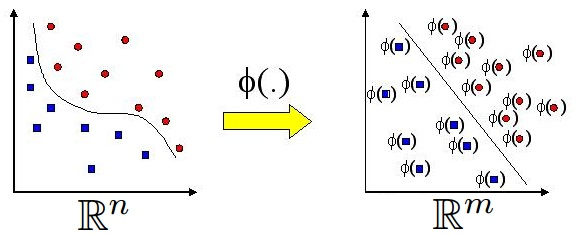
\includegraphics[width=0.4\linewidth]{images/svm-transform-space.jpg}

    \caption{Diagrama de transformación de muestras del espacio vectorial
        $\mathbb{R}^{n}$ a un nuevo espacio $\mathbb{R}^{m}$, con $n \leq m$.}
    \label{fig:ocsvm:svm_transformed_space}
\end{figure}


\subsubsection{Funciones \textit{kernel}}

La transformación de muestras a espacios de mayor dimensión trae consigo
la dificultad de realizar las multiplicaciones de vectores en dichos
espacios. Las multiplicaciones presentes en las ecuaciones
\ref{eq:ocsvm:hyperplane2} y \ref{eq:ocsvm:min_problem_restr2} pueden
provocar que el clasificador consuma demasiados recursos o necesite mucho
tiempo de computación, haciendo que el uso del clasificador en ambientes
reales ya no sea posible
\citep{rieck2009machine}. % from section 3 - kernels (intro paragraph)

Para superar este desafío, se puede emplear unas funciones denominadas
\textit{kernels}, que permiten omitir esas multiplicaciones de vectores
en el nuevo espacio. Los \textit{kernels} comparan dos vectores del
espacio original $\mathbb{R}^{n}$ y retornan un valor escalar que indica
la similitud que dichos vectores presentan en el nuevo espacio
$\mathbb{R}^{m}$ de mayor dimensión.
El resultado producido por estas funciones equivale al producto escalar
de los dos vectores en el nuevo espacio $\mathbb{R}^{m}$, como se
puede observar también en la \autoref{eq:ocsvm:kernel}, pero con la
ventaja de que no se realiza realmente esta multiplicación costosa
\citep{rieck2009machine}. % from section 3.1 - kernels | section 3.2 - geometry

\begin{equation}
    \label{eq:ocsvm:kernel}
    K(\vec{x_{1}}, \vec{x_{2}})
    \ = \
    \phi(\vec{x_{1}}) \cdot \phi(\vec{x_{2}})
\end{equation}

Estos \textit{kernels} no son exclusivos de los clasificadores
\gls{acr3:ocsvm} ni de \gls{acr3:svm}s en general, pero se ha utilizado
estas funciones con mucho éxito en este tipo de clasificadores.
Existen varias opciones de kernels que pueden utilizarse, los más
conocidos son el \textit{kernel} lineal, el polinomial, el sigmoidal
y el \textit{Radial Basis Function} (RBF) \textit{kernel}
\citep{rieck2009machine}. % from section 3.2 - geometry
Usando el \textit{kernel} lineal, el hiperplano separador queda
representado por un hiperplano también en el espacio original; los
otros tres \textit{kernels} mencionados generan superficies no lineales
en el espacio original.
Realizando varias pruebas para comparar la efectividad de estos \textit{kernels},
el \gls{acr3:rbf} es el que arrojó mejores resultados. Además, varios trabajos
relacionados han empleado este \textit{kernel} con éxito para sus tareas
de clasificación, como podemos ver en los trabajos \citep{parhizkar2015oc}
y \citep{perdisci2006using}. Por estos motivos, nosotros utilizamos el
\gls{acr3:rbf} en los clasificadores dentro de nuestro detector
\gls{acr3:name}.
La formulación del \textit{kernel} \gls{acr3:rbf} puede ser expresada
según la \autoref{eq:ocsvm:kernel_rbf}
\citep{parhizkar2015oc}. % from section II.A - one class SVM

\begin{equation}
    \label{eq:ocsvm:kernel_rbf}
    K(\vec{x_{1}}, \vec{x_{2}})
    \ = \
    \phi(\vec{x_{1}}) \cdot \phi(\vec{x_{2}})
    \ = \
    \exp(
        - \gamma \lVert \vec{x_{1}} - \vec{x_{2}} \lVert^2
    )
\end{equation}

En esta ecuación, se puede ver que el \textit{kernel} obtiene el cuadrado
de la norma $l_{2}$ (o distancia euclidiana) de la diferencia de dos
vectores en el espacio original. Este resultado escalar es multiplicado
por un factor $\gamma$, usando este nuevo resultado en una exponenciación
con la base de los logaritmos naturales.
Estas operaciones son computacionalmente más eficientes que la
multiplicación de vectores en espacios de mayores dimensiones
\citep{rieck2009machine}. % from section 3.2 - geometry

En el contexto del \gls{acr3:ocsvm}, el parámetro \gls{sim3:gammai}
determina la dimensión de la región de influencia de cada muestra de
entrenamiento del grupo \gls{sim3:gi}. Esto regula la cercanía necesaria
de nuevas muestras a las muestras de entrenamiento para ser consideradas
pertenecientes a la clase conocida. Este parámetro tiene relación inversa
al radio de la región de influencia de las muestras.
Esto significa que valores menores de \gls{sim3:gammai} aumentan el radio
de la región de influencia de las muestra de entrenamiento, causando que
la superficie separadora que representa al hiperplano en el espacio original
$\mathbb{R}^{n}$ se encuentre más alejada de dichas muestras. En cambio,
valores mayores de \gls{sim3:gammai} reducen este radio de influencia,
permitiendo una superficie más cercana a las muestras vistas.

La \autoref{fig:ocsvm:gamma_values} muestra, con un ejemplo de peticiones
\gls{acr3:http}, la superficie separadora no lineal obtenida en el
espacio original con dos \textit{kernels}. El \gls{acr3:rbf} permite
detectar más anomalías (círculos amarillos) que el \textit{kernel} lineal,
que solamente puede trazar una superficie lineal en el espacio original.
Además, se ilustra la influencia del parámetro \gls{sim3:gammai} en la
forma de la superficie separadora, mostrando que \gls{sim3:gammai} mayor
genera una superficie más ajustada a las muestras de entrenamiento.

\begin{figure}[ht]
    \centering
    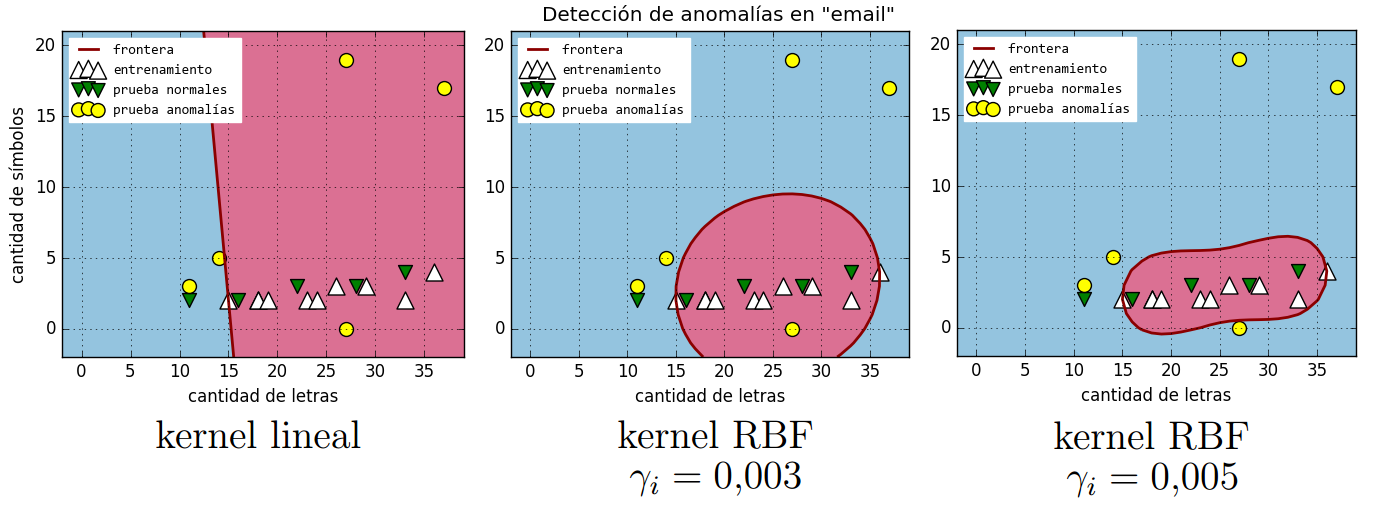
\includegraphics[width=\linewidth]{images/ocsvm-rbf-gamma.png}

    \caption{Comparación de superficies separadoras obtenidas por el
        \gls{acr3:ocsvm} con distintos \textit{kernels} y parámetros.}
    \label{fig:ocsvm:gamma_values}
\end{figure}


\subsubsection{Formulación dual de la optimización}

Para aprovechar la facilidad de cálculo que brindan los \textit{kernels},
es conveniente que el clasificador \gls{acr3:ocsvm} no resuelva directamente
el problema de optimización de la \autoref{eq:ocsvm:min_problem_goal1},
sino que resuelva la formulación dual del problema.
Esta formulación dual queda expresada como se puede observar en la
\autoref{eq:ocsvm:min_problem_dual_goal}, sujeto a las restricciones
que muestra la \autoref{eq:ocsvm:min_problem_dual_restr}
\citep{aggarwal2013outlier}. % from section 3.4 - OCSVM

\begin{equation}
    \label{eq:ocsvm:min_problem_dual_goal}
    \min_{a_{i}}
    \
    \frac{1}{2} \ a_{i} \ S_{i} \ a_{i}^{T}
\end{equation}

\begin{equation}
    \label{eq:ocsvm:min_problem_dual_restr}
    \sum_{j=1}^{\lvert G_{i} \rvert} a_{ij} \ = \ 1
    \ , \quad
    0 \leqslant a_{ij} \leqslant \frac{1}{\nu_{i} \lvert G_{i} \rvert}
    \
    \forall j = 1,2, \dots, \lvert G_{i} \rvert
\end{equation}

En estas ecuaciones, $S_{i}$ es una matriz simétrica que representa los
productos escalares de todas las muestras de entrenamiento multiplicadas
entre ellas en el espacio de dimensiones mayores $\mathbb{R}^{m}$;
ambas dimensiones de esta matriz equivalen a la cantidad de muestras
$\lvert G_{i} \rvert$.
El vector $a_{i}$ contiene una cantidad $\lvert G_{i} \rvert$ de
coeficientes variables que corresponden a cada una de las muestras, y la
formulación dual de la optimización busca encontrar estos coeficientes.
De esta forma, la minimización consta de la multiplicación de un vector
fila $a_{i}$ por una matriz simétrica $S_{i}$, y el vector fila resultante
es multiplicado por el vector columna $a_{i}^{T}$, lo que resulta
finalmente en un valor escalar a ser minimizado.

Las muestras de entrenamiento que tengan coeficiente $a_{ij}$ mayor a
0 serán los vectores de soporte del clasificador. Mayormente, los vectores
de soporte son un subconjunto reducido de las muestras de entrenamiento,
resultando finalmente en un vector $a_{i}$ con la mayoría de los coeficientes
iguales a 0
\citep{perdisci2006using}. % from section 2.1 - OneClassSVM

La matriz simétrica $S_{i}$, que está presente en la formulación dual
de la optimización, representa las multiplicaciones de vectores
que se busca omitir por su alto costo computacional. Esta matriz puede
ser reemplazada por los resultados de un \textit{kernel}. Esto se logra
construyendo una matriz con las mismas dimensiones que $S_{i}$, pero
cuyos elementos son obtenidos mediante un \textit{kernel} en vez de
multiplicación de vectores.

Después de resolver la minimización de la formulación dual, que
presentamos en la \autoref{eq:ocsvm:min_problem_dual_goal}, el clasificador
\gls{acr3:ocsvm} ya tiene disponible el vector de coeficientes $a_{i}$
del grupo \gls{sim3:gi}.
Entonces, el hiperplano definido en la \autoref{eq:ocsvm:hyperplane2}
también puede ser expresado en términos del \textit{kernel} $K_{i}$ que
fue utilizado para sustituir $S_{i}$ en la formulación dual y el vector
$a_{i}$ obtenido por la minimización.

De esta forma, el hiperplano del clasificador puede quedar definido como
lo muestra la \autoref{eq:ocsvm:hyperplane3}
\citep{aggarwal2013outlier}. % from section 3.4 - OCSVM

\begin{equation}
    \label{eq:ocsvm:hyperplane3}
    \vec{w_{i}} \cdot \phi(\vec{x})
    \ - \
    \rho_{i}
    \ = \
    \sum_{j=1}^{\lvert G_{i} \rvert}
    \left(
        a_{ij} \, K_{i}(\vec{f_{ij}}, \vec{x})
    \right)
    \ - \
    \rho_{i}
    \ = \
    0
\end{equation}

Como ya mencionamos, utilizamos el \textit{kernel} \gls{acr3:rbf} en
nuestro \gls{acr3:waf}. Reemplazando la fórmula de este \textit{kernel},
que fue presentada en la \autoref{eq:ocsvm:kernel_rbf}, podemos definir
el hiperplano de la \autoref{eq:ocsvm:hyperplane3} de la forma como lo
expresa la \autoref{eq:ocsvm:hyperplane4}, donde \gls{sim3:gammai} es el
parámetro del \textit{kernel} para el clasificador del grupo \gls{sim3:gi}.

\begin{equation}
    \label{eq:ocsvm:hyperplane4}
    \vec{w_{i}} \cdot \phi(\vec{x})
    \ - \
    \rho_{i}
    \ = \
    \sum_{j=1}^{\lvert G_{i} \rvert}
    \left(
        a_{ij} \,
        \exp(
            - \gamma_{i} \lVert \vec{f_{ij}} - \vec{x} \lVert^2
        )
    \right)
    \ - \
    \rho_{i}
    \ = \
    0
\end{equation}

De esta forma, el clasificador \gls{acr3:ocsvm} puede construir un
hiperplano separador a través de la simulación de multiplicación de
vectores en espacios de altas dimensiones, pero sin incurrir
realmente en los elevados costos computacionales que implicaría la
realización de esas multiplicaciones.


\subsection{Fase de detección}

Después de la fase de entrenamiento, el clasificador \gls{acr3:ocsvm}
está preparado para clasificar nuevas muestras, analizando de que lado
del hiperplano se encuentran las mismas. Si están situadas en el lado
opuesto al origen, serán consideradas como pertenecientes a la clase
conocida. En caso contrario, no pertenecerán a dicha clase
\citep{perdisci2006using}. % from section 2.1 - OneClassSVM
En nuestro contexto de detección de anomalías, el \gls{acr3:waf} representa
cada nueva petición \gls{acr3:http} con un vector de \textit{features}
con dimensiones correspondientes al grupo \gls{sim3:gi} según método y
\gls{acr3:url} de la petición. Luego se analiza la posición de ese vector
con respecto al hiperplano trazado por el clasificador del grupo.

En esta fase de detección, el clasificador \gls{acr3:ocsvm} emplea la
fórmula del hiperplano en una función de decisión con el fin de determinar
si una muestra nueva pertenece a la clase conocida o no. En la
\autoref{eq:ocsvm:decision1} se puede observar la formulación de esta
función de decisión en términos del hiperplano
\citep{amer2013paper}. % from section 3.1 - Motivation of OneClassSVM

\begin{equation}
    \label{eq:ocsvm:decision1}
    g_{i}(\vec{x})
    \ = \
    \begin{cases}
        \vec{w_{i}} \cdot \vec{x} - \rho_{i} \ \geqslant \ 0    & +1 \\
        \text{caso contrario}                                   & -1
    \end{cases}
\end{equation}

En esta ecuación, \gls{sim3:wi} es el vector que define el hiperplano
del grupo, $\vec{x}$ es el vector que representa las nuevas muestras a
analizar, \gls{sim3:rhoi} es la distancia del hiperplano al origen y
$g_{i}(\vec{x})$ es la función de decisión, que recibe el vector $\vec{x}$
como su argumento.
De esta forma, se obtendrá $g_{i}(\vec{x}) = 1$ para las muestras que se
encuentran separadas del origen por el hiperplano, indicando que las mismas
pertenecen a la clase conocida, pero se tendrá $g_{i}(\vec{x}) = -1$ para
las muestras que se encuentren en el mismo lado que el origen, indicando
que estas últimas no pertenecen a dicha clase.

En el contexto de nuestro \gls{acr3:waf}, nuevas peticiones \gls{acr3:http}
serán representadas por vectores de \textit{features} $\vec{x}$, siempre
atendiendo que las dimensiones de esos vectores sean correspondientes a
sus grupo \gls{sim3:gi} respectivos.
La función $g_{i}(\vec{x})$ retorna el valor positivo para peticiones
detectadas como normales (que serán identificadas como muestras negativas)
y devuelve el valor negativo para aquellas peticiones detectadas como
anomalías (que serán identificadas como muestras positivas o ataques).

Para vectores en espacios de dimensiones mayores, esta función de decisión
incorpora las ya mencionadas funciones de transformación $\phi$, y puede
ser expresada de la forma que lo indica la \autoref{eq:ocsvm:decision2}
\citep{amer2013paper}. % from section 3.1 - Motivation of OneClassSVM

\begin{equation}
    \label{eq:ocsvm:decision2}
    g_{i}(\vec{x})
    \ = \
    \begin{cases}
        \vec{w_{i}} \cdot \phi(\vec{x}) - \rho_{i} \ \geqslant \ 0  & +1 \\
        \text{caso contrario}                                       & -1
    \end{cases}
\end{equation}

Empleando las optimizaciones que nos brindan los \textit{kernels}, podemos
sustituir la multiplicación de vectores en esta función. De esta forma,
la función de decisión que expresada según la \autoref{eq:ocsvm:decision3}
\citep{perdisci2006using}. % from section 2.1 - OneClassSVM

\begin{equation}
    \label{eq:ocsvm:decision3}
    g_{i}(\vec{x})
    \ = \
    \begin{cases}
        \sum_{j=1}^{\lvert G_{i} \rvert}
        \left(
            a_{ij} \, K_{i}(\vec{f_{ij}}, \vec{x})
        \right)
        - \rho_{i} \ \geqslant \ 0  & +1 \\
        \text{caso contrario}       & -1
    \end{cases}
\end{equation}

Finalmente, reemplazando en esta ecuación la fórmula del \textit{kernel}
\gls{acr3:rbf}, obtenemos una función según la \autoref{eq:ocsvm:decision4},
donde $\gamma_{i}$ es el parámetro del \textit{kernel} para el
clasificador del grupo \gls{sim3:gi} correspondiente.

\begin{equation}
    \label{eq:ocsvm:decision4}
    g_{i}(\vec{x})
    \ = \
    \begin{cases}
        \sum_{j=1}^{\lvert G_{i} \rvert}
        \left(
            a_{ij} \,
            \exp(
                - \gamma_{i} \lVert \vec{f_{ij}} - \vec{x} \lVert^2
            )
        \right)
        - \rho_{i} \ \geqslant \ 0  & +1 \\
        \text{caso contrario}       & -1
    \end{cases}
\end{equation}

Se puede observar que la función de decisión, que se utiliza para determinar
de que lado del hiperplano cae una nueva muestra, se reduce a calcular
la norma $l_{2}$ entre la muestra nueva y los vectores de soporte (aquellos
con coeficientes $a_{ij}$ mayor a 0). Considerando que suele haber una
cantidad reducida de vectores de soporte en un clasificador entrenado,
esta función de decisión $g_{i}(\vec{x})$ resulta en computaciones rápidas
y eficientes \citep{perdisci2006using}. % from section 2.1 - OneClassSVM
De esta manera mostramos que el clasificador \gls{acr3:ocsvm} es una
herramienta con un bajo costo computacional durante la fase de detección,
y por lo tanto puede ser empleado en nuestro detector \gls{acr3:name}
para realizar la detección en tiempo real de mensajes \gls{acr3:http}
anómalos.


\section{Trabajos relacionados con One-Class SVM}

En la sección anterior describimos el funcionamiento del clasificador
\gls{acr3:ocsvm}, mostrando las ecuaciones que definen su comportamiento
durante las fases de entrenamiento y detección.
A continuación presentamos algunos trabajos relacionados del área de
\gls{acr3:ids} que utilizan este clasificador.

En \citep{nguyen2016pocad} se presenta un detector llamado \textit{POCAD}.
Este detector extrae conjuntos de \textit{n-grams} de \textit{bytes} de
paquetes \gls{acr3:ip} y peticiones \gls{acr3:http} y luego aplica un
proceso de \textit{clustering} para reducir la cantidad de \textit{features};
\gls{acr3:name} utiliza los procesos de extracción de \textit{features}
presentados en el \autoref{chap:p3_concepts_features}, que no incluyen
\textit{n-grams}.
Posteriormente, \textit{POCAD} utiliza un \gls{acr3:ocsvm} para realizar
la detección de anomalías, de manera similar a nuestra implementación.
Los autores realizan pruebas comparativos con otros sistemas de detección,
concluyendo que su implementación logra una mejor detección que los demás.

En \citep{parhizkar2015oc} se presenta un detector de anomalías llamado
\textit{OC-WAD} para peticiones \gls{acr3:http}. Los autores extraen
una cantidad fija de \textit{features} de las peticiones, a diferencia
de nuestros procesos de extracción que producen una cantidad variable
de \textit{features} que depende de los parámetros presentes en las
peticiones.
Posteriormente, \textit{OC-WAD} utiliza un conjunto de \gls{acr3:ocsvm}
con \textit{kernel} \gls{acr3:rbf} para realizar la detección, poniendo
énfasis en la creación y optimización del conjunto de clasificadores
mediante un algoritmo de enjambres llamado \textit{BeeSnips}.
Nuestro \gls{acr3:name} utiliza también el mismo \textit{kernel} y
clasificador, pero se entrena un clasificador por grupo de método y
\gls{acr3:url}.
Los autores concluyen mediante algunas comparaciones que su implementación
supera algunos otros trabajos que mencionan.

En \citep{perdisci2006using} presentan un detector que extrae conjuntos
de \textit{n-grams} de \textit{bytes} de peticiones \gls{acr3:http}.
También se aplica un proceso de \textit{clustering} sobre los \textit{features}
extraídos. Como ya explicamos, nuestros procesos de extracción no analizan
\textit{n-grams}.
Los autores emplean un conjunto de \gls{acr3:ocsvm} con el \textit{kernel}
\gls{acr3:rbf}; cada uno de los clasificadores es entrenado sobre distintos
subconjuntos de \textit{features}. En cambio, \gls{acr3:name} utiliza
también el mismo \textit{kernel} y clasificador, pero se entrena un
clasificador por grupo de método y \gls{acr3:url}.
Las conclusiones de los autores subrayan la robustez de su detector
frente a ataques que tratan de ocultar su firma utilizando diversas
técnicas de ofuscación.

En \citep{tran2004one} se presenta un detector de anomalías llamado
\textit{OTAD} para analizar paquetes \gls{acr3:ip}. Los autores utilizan
una cantidad fija de cinco \textit{features} que corresponden a datos
obtenidos mediante la herramienta \textit{tcpstat}; nuestra implementación
extrae una cantidad variable de \textit{features} de peticiones
\gls{acr3:http}.
Posteriormente, \textit{OTAD} emplea un clasificador \gls{acr3:ocsvm}
con el \textit{kernel} \gls{acr3:rbf}, utilizando un algoritmo genético
para la optimización de la selección de parámetros. En cambio, \gls{acr3:name}
utiliza también el mismo \textit{kernel} y clasificador, pero sin mecanismo
para la selección automática de parámetros.
Los autores concluyen que su detector obtiene buenos resultados, con la
ventaja de poder utilizar directamente los datos del \textit{tcpstat}
sin necesidad de conversiones o transformaciones.

En \citep{rieck2009machine} se propone un detector de anomalías que trabaja
sobre un conjunto variado de \textit{features} de peticiones \gls{acr3:http},
incluyendo secuencias y árboles para representar relaciones en los datos.
Emplea un tipo de \gls{acr3:ocsvm} que esta implementado de forma distinta
a lo que presentamos en este capítulo; el autor usa un clasificador que
emplea una hiperesfera en vez de un hiperplano para clasificar las muestras.
Concluye que el detector presentado detecta una gran variedad de ataques,
resaltando la baja tasa de falsos positivos.

El éxito en la detección de anomalías que reportan estos trabajos nos
confirma que el clasificador \gls{acr3:ocsvm} es una herramienta útil
para nuestro \gls{acr3:waf}.


\section{Clasificación de peticiones de ejemplo}

Después de haber explicado el funcionamiento del clasificador \gls{acr3:ocsvm},
a continuación ilustramos el proceso de clasificación y detección de
anomalías \gls{acr3:http} que realiza nuestro detector \gls{acr3:name}.
En el \autoref{chap:p3_concepts_features} hemos introducido un ejemplo
mediante el cual explicamos nuestros procesos de extracción de \textit{features}.
En la \autoref{tbl:fe:example_1} se pudo observar 20 peticiones de ejemplo,
con las cuales realizamos la extracción y el escalamiento de los
\textit{features}. Los números finales que representan las peticiones
fueron presentados en las tablas \ref{tbl:fe:example_scaled_whole_req},
\ref{tbl:fe:example_scaled_email} y \ref{tbl:fe:example_scaled_full}.

Para el proceso de clasificación, entrenamos un \gls{acr3:ocsvm} con la
matriz \gls{sim3:mi} obtenida a partir de nuestras peticiones de ejemplo,
la cual tiene 10 filas y 30 columnas.
Para la selección de los valores para \gls{sim3:nui} y \gls{sim3:gammai}
realizamos el entrenamiento con varios valores en el rango
$[\num{0.0001} ; \num{0.5}]$, seleccionando los valores con los mejores
resultados en la fase de detección. De esta forma, para este ejemplo
utilizamos los valores \num{0.2778} y \num{0.0001} para \gls{sim3:nui}
y \gls{sim3:gammai} respectivamente.

\begin{table}[ht]
    \centering
    \small
    \begin{tabularx}{\linewidth}{|c|C|C|C|C|C|}
        \hline
        ID & Grupo         & Vector de soporte & Clasificación real & Clasificación obtenida & Correctamente clasificado \\ \specialrule{1.5pt}{0}{0}
         1 & entrenamiento & -                 & normal             & normal                 & Sí                        \\ \hline
         2 & entrenamiento & -                 & normal             & normal                 & Sí                        \\ \hline
         3 & entrenamiento & -                 & normal             & normal                 & Sí                        \\ \hline
         4 & entrenamiento & -                 & normal             & normal                 & Sí                        \\ \hline
         5 & entrenamiento & Sí                & normal             & normal                 & Sí                        \\ \hline
         6 & entrenamiento & -                 & normal             & normal                 & Sí                        \\ \hline
         7 & entrenamiento & Sí                & normal             & normal                 & Sí                        \\ \hline
         8 & entrenamiento & Sí                & normal             & normal                 & Sí                        \\ \hline
         9 & entrenamiento & Sí                & normal             & normal                 & Sí                        \\ \hline
        10 & entrenamiento & -                 & normal             & normal                 & Sí                        \\ \hline
        11 & detección     & -                 & normal             & normal                 & Sí                        \\ \hline
        12 & detección     & -                 & normal             & normal                 & Sí                        \\ \hline
        13 & detección     & -                 & normal             & anomalía               & -                         \\ \hline
        14 & detección     & -                 & normal             & anomalía               & -                         \\ \hline
        15 & detección     & -                 & normal             & normal                 & Sí                        \\ \hline
        16 & detección     & -                 & anomalía           & anomalía               & Sí                        \\ \hline
        17 & detección     & -                 & anomalía           & anomalía               & Sí                        \\ \hline
        18 & detección     & -                 & anomalía           & anomalía               & Sí                        \\ \hline
        19 & detección     & -                 & anomalía           & anomalía               & Sí                        \\ \hline
        20 & detección     & -                 & anomalía           & anomalía               & Sí                        \\ \hline
    \end{tabularx}

    \caption{Resultados de clasificación de nuestras 20 peticiones de
        ejemplo.}
    \label{tbl:ocsvm:example}
\end{table}

En la \autoref{tbl:ocsvm:example} se pueden observar los resultados del
entrenamiento y la posterior detección de todas las peticiones de ejemplo.
Se puede notar que, como se ha explicado en este capítulo, solamente
algunas de las muestras de entrenamiento (que son las primeras 10 peticiones)
son utilizados como vectores de soporte del clasificador.
Además, la tabla muestra que 18 de las 20 peticiones fueron clasificadas
correctamente por el \gls{acr3:ocsvm} entrenado; solamente dos peticiones
normales fueron categorizadas incorrectamente, mientras que las cinco
anomalías del conjunto de ejemplo fueron detectadas por el clasificador.

Como muestran los resultados, la clasificación no siempre es exitosa,
ya que depende de las muestras con las que debe trabajar el clasificador.
No podemos visualizar en dos o tres dimensiones el espacio original de
30 \textit{features}, ni mucho menos el espacio de dimensiones superiores.
De esta forma, no hemos logrado analizar la superficie separadora que
representa al hiperplano en el espacio original; el análisis de las
componentes principales (PCA) tampoco pudo brindar aportes en este análisis.
La idea de este ejemplo es también resaltar esta realidad en las tareas
de detección de anomalías, mostrando una situación en la cual no se logra
la detección correcta de todas las muestras.

\begin{figure}[ht]
    \centering
    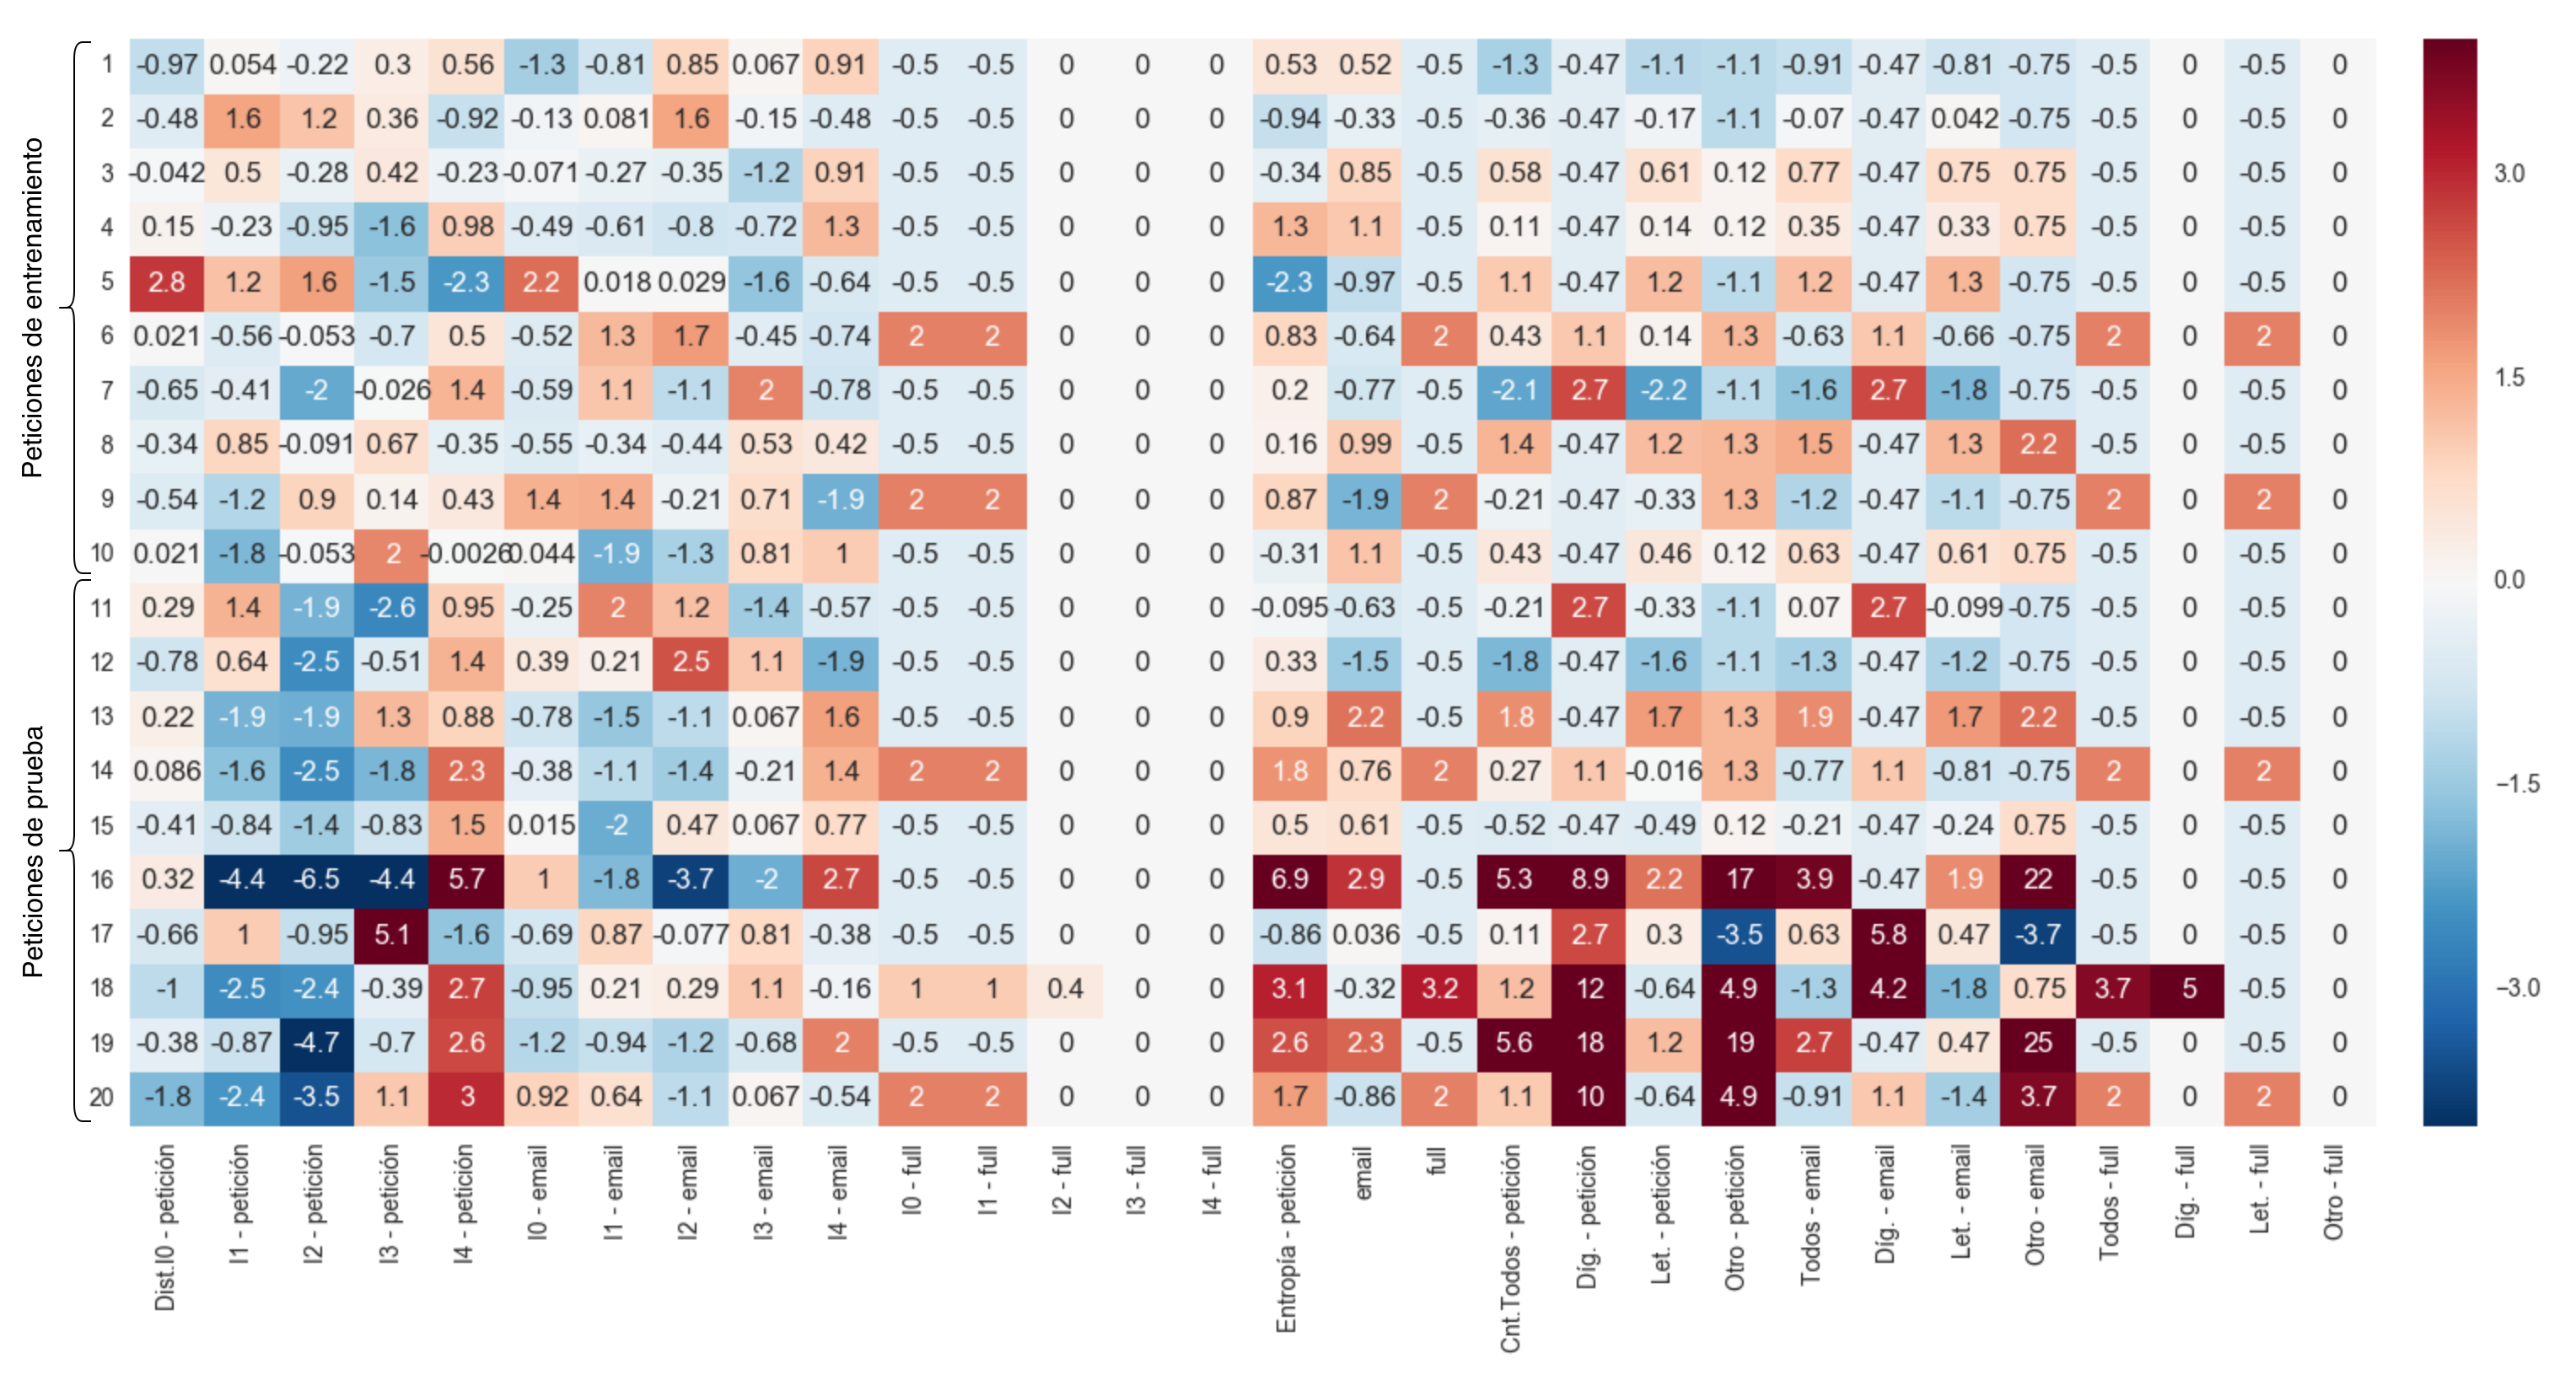
\includegraphics[width=\linewidth]{images/example-features-heatmap.png}

    \caption{Mapa de calor de los \textit{features} extraídos de nuestras
        20 peticiones de ejemplo.}
    \label{fig:ocsvm:example_heatmap}
\end{figure}

En la \autoref{fig:ocsvm:example_heatmap} se puede observar los números
escalados de todos nuestros \textit{features} para las 20 peticiones de
ejemplo, desplegadas dentro de un gráfico del tipo mapa de calor
(\textit{heatmap}) para permitir una mejor visualización de los rangos
de valores. Cada \textit{features} fue escalado para que su promedio sea 0,
que en el gráfico corresponde al color blanco; regiones de colores rojo o
azul oscuros indican mayor alejamiento del 0.
Se puede notar, por ejemplo, que las peticiones 16 al 20, que contienen
anomalías, tienen mayores ocurrencias de colores oscuros que indican que
esos \textit{features} están alejados del promedio; esto le permite al
\gls{acr3:ocsvm} detectar estas anomalías.

En cambio, la petición 14 tiene un valor mucho más elevado para el último
intervalo de la distribución de caracteres de la petición completa
(quinta columna desde la izquierda) que todas las peticiones de entrenamiento,
lo que pudo haber provocado que el clasificador no detectó esa petición
como normal. Lo mismo se da para la petición 13, que tiene una entropía
del parámetro \textit{email} más elevada que las peticiones de entrenamiento.

Esta representación de los \textit{features} puede ser de utilidad para
continuar el análisis de los datos, inspeccionando las relaciones entre
los \textit{features} extraídos y los resultados de clasificación
mostrados en la \autoref{tbl:ocsvm:example}.
